\documentclass[12pt, a4paper]{article}

\usepackage[utf8]{inputenc}
\usepackage{graphicx}
\usepackage[T1]{fontenc}
\usepackage{babel}
\usepackage{amsmath}
\usepackage{amssymb}
\usepackage{geometry}
\usepackage{booktabs}
\usepackage{hyperref}
\usepackage{float}
\usepackage[hypcap=false]{caption}

% Para los bloques CML-DEVS usamos alltt
\usepackage{alltt}
\usepackage{xcolor}

\geometry{
    top=2.5cm,
    bottom=2.5cm,
    left=3cm,
    right=3cm
}

% Comandos de conveniencia para CML-DEVS
\newcommand{\cmlgt}{$>$}
\newcommand{\cmlle}{$\leq$}
\newcommand{\cmleq}{$=$}
\newcommand{\cmlplus}{$+$}
\newcommand{\cmlN}{$\mathbb{N}$}
\newcommand{\cmlgeq}{$\geq$}
\newcommand{\cmllt}{$<$}
\newcommand{\cmlwedge}{$\wedge$}
\newcommand{\cmlneq}{$\neq$}
\newcommand{\cmlvee}{$\vee$}
\newcommand{\kw}[1]{\textbf{#1}}
\newcommand{\cmlR}{$\mathbb{R}$}
\newcommand{\cmlTime}{\textbf{Time}}
\newcommand{\cmlsigma}{$\sigma$}
\newcommand{\dint}{$\delta_{\mathit{int}}$}
\newcommand{\dext}{$\delta_{\mathit{ext}}$}
\newcommand{\clambda}{$\lambda$}
\newcommand{\cmlta}{\textbf{ta}}
\newcommand{\cmlcomment}[1]{\textit{\textcolor{gray}{#1}}}

\newenvironment{cmldevs}{%
  \begin{alltt}\small%
}{%
  \end{alltt}%
}

% ----------------------------------------------------------------

\title{
    \large Simulación de Sistemas \\[0.5em]
    \LARGE \textbf{Proyecto de Simulación} \\[0.3em]
    \large Sistema de Tiempo Real: Controlador Simplificado de Bomba de Infusión \\[1em]
    \normalsize Especificación DEVS de los Modelos Atómicos
}

\author{
    Jhonatan Calle Galeano \and Hernan Jara
}

\date{}

% ================================================================
\begin{document}
\maketitle
\thispagestyle{empty}

% ----------------------------------------------------------------
\section{Generador de Órdenes Médicas}

El modelo \textbf{GeneradorOrdenes} es un modelo atómico autónomo (sin entradas)
que genera periódicamente eventos \texttt{ordenMedica}, indicando el caudal objetivo
que debe administrar la bomba. Las órdenes pueden generarse de manera determinística
(caudal y tiempo entre órdenes fijos) o estocástica (caudal con distribución gaussiana,
interarribo con distribución exponencial) según los escenarios definidos en
\texttt{config.py}.

\begin{center}
\begin{cmldevs}
\kw{atomic} GeneradorOrdenes \kw{is} <Y, S, \dint{}, \clambda{}, \cmlta{}> \kw{where}
\kw{S is}
    caudalProximo : \cmlR{};    \cmlcomment{-- caudal objetivo (0 a 200 ml/h)}
    interarribo   : \cmlTime{};  \cmlcomment{-- tiempo hasta la siguiente orden}
    \cmlsigma{}             : \cmlTime{};  \cmlcomment{-- variable de avance de tiempo}
\kw{end S}
\kw{Y is}
    ordenMedica : \cmlR{};      \cmlcomment{-- puerto de salida: valor del caudal}
\kw{end Y}
\dint{}(caudalProximo, interarribo, \cmlsigma{}) \kw{is}
    \cmlcomment{-- Deterministico: valores fijos del config}
    \cmlcomment{-- Estocastico: caudal ~ Gauss(media, desvio), interarribo ~ Exp(media)}
    caudalProximo = next\_caudal\_logic();
    interarribo   = next\_interarribo\_logic();
    \cmlsigma{}   = interarribo;
\kw{end} \dint{}
\clambda{}(caudalProximo, interarribo, \cmlsigma{}) \kw{is}
    ordenMedica = caudalProximo;
\kw{end} \clambda{}
\cmlta{}(caudalProximo, interarribo, \cmlsigma{}) \kw{is}
    \cmlsigma{};
\kw{end} \cmlta{}
\kw{end atomic}
\end{cmldevs}
\captionof{figure}{Especificación CML-DEVS: Generador de Órdenes Médicas}
\label{fig:generador-ordenes}
\end{center}

\subsection*{Análisis del modelo}

\begin{enumerate}
    \item \textbf{Modos de generación}: En modo determinístico, \texttt{caudal\_fijo}
    e \texttt{interarribo\_fijo} provienen del \texttt{config.py}. En modo estocástico,
    el caudal se muestrea de una distribución Gaussiana acotada a $[0, 200]$ ml/h y
    el tiempo entre órdenes de una distribución Exponencial.

    \item \textbf{Estado inicial}: Se inicializa con el primer caudal y el primer
    interarribo calculados en el constructor, de modo que la primera emisión ocurre
    exactamente al tiempo \texttt{interarribo\_fijo} (o su equivalente estocástico).
\end{enumerate}


% ----------------------------------------------------------------
\section{Sensor de Flujo}

El modelo \textbf{SensorFlujo} reporta periódicamente el caudal real cada
\texttt{PERIODO\_SENSOR} segundos (definido en \texttt{config.py}, por defecto 1\,s).
Al recibir \texttt{caudalActual} del actuador, incorpora ese valor y modela una deriva
física proporcional al tiempo transcurrido sin actualización, más un ruido gaussiano
opcional.

\begin{center}
\begin{cmldevs}
\kw{atomic} SensorFlujo \kw{is} <X, Y, S, \dint{}, \dext{}, \clambda{}, \cmlta{}> \kw{where}
\kw{S is}
    caudalMedido    : \cmlR{};     \cmlcomment{-- valor de caudal a reportar}
    caudalActuador  : \cmlR{};     \cmlcomment{-- ultimo valor recibido del actuador}
    tiempoActuador  : \cmlTime{};  \cmlcomment{-- tiempo acumulado desde ultima actualizacion}
    \cmlsigma{}               : \cmlTime{}; \cmlcomment{-- controla el periodo de muestreo}
\kw{end S}
\kw{X is}
    caudalActual : \cmlR{};  \cmlcomment{-- caudal fisico recibido del actuador}
\kw{end X}
\kw{Y is}
    sensorFlujo  : \cmlR{};  \cmlcomment{-- medicion enviada al Controlador}
\kw{end Y}
\dext{}((caudalMedido, caudalActuador, tiempoActuador, \cmlsigma{}), e, (puerto, valor)) \kw{is}
    \cmlsigma{}     = max(0.0, \cmlsigma{} - e);
    caudalActuador  = valor;
    caudalMedido    = valor;   \cmlcomment{-- actualizacion inmediata del valor medido}
    tiempoActuador  = 0.0;
        \kw{if} (puerto = caudalActual)
\kw{end} \dext{}
\dint{}(caudalMedido, caudalActuador, tiempoActuador, \cmlsigma{}) \kw{is}
    \cmlcomment{-- deriva = caudalActuador * TASA\_DERIVA * tiempoActuador}
    \cmlcomment{-- ruido  ~ Gauss(0, ruido\_std)  si ruido\_std > 0}
    caudalMedido   = max(0.0, caudalActuador + deriva + ruido);
    tiempoActuador = tiempoActuador + \cmlsigma{};
    \cmlsigma{}    = PERIODO\_SENSOR;
\kw{end} \dint{}
\clambda{}(caudalMedido, caudalActuador, tiempoActuador, \cmlsigma{}) \kw{is}
    sensorFlujo = caudalMedido;
\kw{end} \clambda{}
\cmlta{}(caudalMedido, caudalActuador, tiempoActuador, \cmlsigma{}) \kw{is}
    \cmlsigma{};
\kw{end} \cmlta{}
\kw{end atomic}
\end{cmldevs}
\captionof{figure}{Especificación CML-DEVS: Sensor de Flujo}
\label{fig:sensor-flujo}
\end{center}

\subsection*{Análisis del modelo}

\begin{enumerate}
    \item \textbf{Frecuencia de muestreo} ($\mathit{ta}$ y $\delta_{\mathit{int}}$):
    El sensor reporta el caudal cada \texttt{PERIODO\_SENSOR} segundos.
    $\sigma$ se resetea a \texttt{PERIODO\_SENSOR} en cada transición interna.

    \item \textbf{Incorporación del valor del actuador} ($\delta_{\mathit{ext}}$):
    Al recibir \texttt{caudalActual}, el modelo actualiza \texttt{caudalActuador}
    y \texttt{caudalMedido} de forma inmediata, resetea \texttt{tiempoActuador} a
    $0.0$ y avanza el cronograma con $\sigma = \max(0, \sigma - e)$.

    \item \textbf{Deriva y ruido} ($\delta_{\mathit{int}}$):
    La medición incorpora una \emph{deriva} proporcional al caudal base y al tiempo
    sin actualización (\texttt{TASA\_DERIVA\_SENSOR} $\times$ \texttt{tiempoActuador}),
    más un \emph{ruido} gaussiano de desviación estándar \texttt{ruido\_std}
    (configurable por escenario; $0$ lo desactiva).

    \item \textbf{Estado inicial}: \texttt{caudalMedido} $= 0.0$,
    \texttt{caudalActuador} $= 0.0$, \texttt{tiempoActuador} $= 0.0$,
    $\sigma = \texttt{PERIODO\_SENSOR}$.
\end{enumerate}

% ----------------------------------------------------------------
\section{Actuador de la Bomba}

El modelo \textbf{ActuadorBomba} representa la interfaz física de la bomba: recibe
comandos lógicos del controlador y, tras una latencia de \texttt{LATENCIA\_ACTUADOR}
segundos (constante importada de \texttt{config.py}, por defecto 0.5\,s), actualiza
el caudal real suministrado al paciente. Incorpora un \texttt{factor\_falla}
configurable que simula degradación mecánica.

\begin{center}
\begin{cmldevs}
\kw{atomic} ActuadorBomba \kw{is} <X, Y, S, \dint{}, \dext{}, \clambda{}, \cmlta{}> \kw{where}

\kw{S is}
    caudalFisico   : \cmlR{};       \cmlcomment{-- caudal que actualmente sale de la bomba}
    caudalObjetivo : \cmlR{};       \cmlcomment{-- caudal a alcanzar tras la latencia}
    \cmlsigma{}            : \cmlTime{};    \cmlcomment{-- controla la latencia (LATENCIA\_ACTUADOR)}
\kw{end S}

\kw{X is}
    ajustarCaudal : \cmlR{};        \cmlcomment{-- nuevo valor de dosis desde el controlador}
    detenerBomba  : \{signal\};     \cmlcomment{-- senal de parada de emergencia}
\kw{end X}

\kw{Y is}
    caudalActual : \cmlR{};         \cmlcomment{-- notifica el cambio fisico al Sensor}
\kw{end Y}

\dext{}((caudalFisico, caudalObjetivo, \cmlsigma{}), e, (puerto, valor)) \kw{is}
    \kw{defcases}
        caudalObjetivo = valor;   \cmlsigma{} = LATENCIA\_ACTUADOR;
            \kw{if} (puerto = ajustarCaudal)
        caudalObjetivo = 0.0;     \cmlsigma{} = LATENCIA\_ACTUADOR;
            \kw{if} (puerto = detenerBomba)
    \kw{end defcases}
\kw{end} \dext{}

\dint{}(caudalFisico, caudalObjetivo, \cmlsigma{}) \kw{is}
    caudalFisico = caudalObjetivo * factor\_falla;
    \cmlsigma{}          = infinity;
\kw{end} \dint{}

\clambda{}(caudalFisico, caudalObjetivo, \cmlsigma{}) \kw{is}
    \cmlcomment{-- Aplica factor\_falla al emitir (simula degradacion mecanica)}
    caudalActual = round(caudalObjetivo * factor\_falla, 3);
\kw{end} \clambda{}

\cmlta{}(caudalFisico, caudalObjetivo, \cmlsigma{}) \kw{is}
    \cmlsigma{};
\kw{end} \cmlta{}

\kw{end atomic}
\end{cmldevs}
\captionof{figure}{Especificación CML-DEVS: Actuador de la Bomba}
\label{fig:actuador-bomba}
\end{center}

\subsection*{Análisis del modelo}

\begin{enumerate}
    \item \textbf{Latencia configurable}: La constante \texttt{LATENCIA\_ACTUADOR}
    se importa de \texttt{config.py} (valor por defecto: 0.5\,s). Ambas ramas de
    $\delta_{\mathit{ext}}$ la aplican, garantizando que todo cambio de caudal,
    incluyendo la parada de emergencia, experimenta el mismo retardo físico.

    \item \textbf{Factor de falla} (\texttt{factor\_falla}): Parámetro configurable
    por escenario (\texttt{config["actuador"]["factor\_falla"]}). Un valor de
    $1.0$ indica funcionamiento nominal; valores inferiores simulan degradación
    mecánica. Se aplica tanto en $\lambda$ (notificación al sensor) como en
    $\delta_{\mathit{int}}$ (actualización del estado físico interno).

    \item \textbf{Estado pasivo}: Cuando no hay órdenes pendientes, $\sigma = \infty$.
    El actuador mantiene el caudal actual indefinidamente hasta que el controlador
    envíe un nuevo evento.

    \item \textbf{Sincronización con el sensor}: La salida \texttt{caudalActual}
    se conecta en el modelo acoplado a la entrada del Sensor de Flujo.
\end{enumerate}

% ----------------------------------------------------------------
\section{Módulo de Alarmas}

El modelo \textbf{ModuloAlarmas} gestiona las notificaciones hacia el personal médico,
emitiendo alertas y manteniendo un ciclo de retransmisión para las alarmas críticas
no confirmadas. Los tiempos de espera y repetición (\texttt{TIEMPO\_CONF\_CRITICA} y
\texttt{PERIODO\_REP\_CRITICA}) se importan de \texttt{config.py}.

\begin{center}
\begin{cmldevs}
\kw{atomic} ModuloAlarmas \kw{is} <X, Y, S, \dint{}, \dext{}, \clambda{}, \cmlta{}> \kw{where}
\kw{S is}
    tipoAlarma : \{BAJA, MEDIA, CRITICA, NINGUNA\};
    fase       : \{OCIOSO, NOTIFICANDO, ESPERANDO\_CONF, REPETIENDO\};
    \cmlsigma{}      : \cmlTime{}; \cmlcomment{-- control del tiempo de avance}
\kw{end S}
\kw{X is}
    alarma                : \{baja, media, critica\}; \cmlcomment{-- niveles de alarma}
    confirmacionEnfermero : \{signal\};               \cmlcomment{-- confirmacion manual}
\kw{end X}
\kw{Y is}
    notificacionAlarma : \kw{Text}; \cmlcomment{-- mensaje hacia el entorno exterior}
\kw{end Y}
\dext{}((tipoAlarma, fase, \cmlsigma{}), e, (puerto, valor)) \kw{is}
    \cmlsigma{} = max(0.0, \cmlsigma{} - e);
    \kw{defcases}
        tipoAlarma = NINGUNA; fase = OCIOSO; \cmlsigma{} = infinity;
            \kw{if} (puerto = confirmacionEnfermero)
        \cmlcomment{-- Filtro de prioridad: CRITICA no es reemplazada}
        \cmlcomment{-- MEDIA no es reemplazada por BAJA}
        tipoAlarma = valor; fase = NOTIFICANDO; \cmlsigma{} = 0.0;
            \kw{if} (puerto = alarma \cmlwedge{} tipoAlarma \cmlneq{} CRITICA
                \cmlwedge{} \kw{not}(tipoAlarma = MEDIA \cmlwedge{} valor = baja))
    \kw{end defcases}
\kw{end} \dext{}
\dint{}(tipoAlarma, fase, \cmlsigma{}) \kw{is}
    \kw{defcases}
        fase = ESPERANDO\_CONF; \cmlsigma{} = TIEMPO\_CONF\_CRITICA;
            \kw{if} (tipoAlarma = CRITICA \cmlwedge{} fase = NOTIFICANDO)
        fase = REPETIENDO; \cmlsigma{} = PERIODO\_REP\_CRITICA;
            \kw{if} (tipoAlarma = CRITICA \cmlwedge{}
            (fase = ESPERANDO\_CONF \cmlvee{} fase = REPETIENDO))
        tipoAlarma = NINGUNA; fase = OCIOSO; \cmlsigma{} = infinity;
            \kw{if} (tipoAlarma = MEDIA \cmlvee{} tipoAlarma = BAJA)
    \kw{end defcases}
\kw{end} \dint{}
\clambda{}(tipoAlarma, fase, \cmlsigma{}) \kw{is}
    notificacionAlarma = "ALERTA: " \cmlplus{} tipoAlarma;
\kw{end} \clambda{}
\cmlta{}(tipoAlarma, fase, \cmlsigma{}) \kw{is}
    \cmlsigma{};
\kw{end} \cmlta{}
\kw{end atomic}
\end{cmldevs}
\captionof{figure}{Especificación CML-DEVS: Módulo de Alarmas}
\label{fig:modulo-alarmas}
\end{center}

\subsection*{Análisis del modelo}

\begin{enumerate}
    \item \textbf{Prioridad de alarmas} ($\delta_{\mathit{ext}}$):
    Se implementó un filtro jerárquico: una alarma \texttt{CRITICA} activa no puede
    ser reemplazada por ninguna otra, y una alarma \texttt{MEDIA} activa no es
    reemplazada por una \texttt{BAJA}. La confirmación del enfermero siempre tiene
    prioridad y limpia cualquier estado.

    \item \textbf{Estados transitorios} ($ta = 0$): Al recibir una nueva alarma que
    pasa el filtro, la $\delta_{\mathit{ext}}$ asigna $\sigma = 0$, forzando la
    ejecución inmediata de $\lambda$.

    \item \textbf{Lógica de repetición crítica}: Tras la primera notificación,
    $\delta_{\mathit{int}}$ transiciona a \texttt{ESPERANDO\_CONF} con
    $\sigma = \texttt{TIEMPO\_CONF\_CRITICA}$ (30\,s). Si no llega confirmación,
    pasa al estado \texttt{REPETIENDO} con ciclos de $\sigma = \texttt{PERIODO\_REP\_CRITICA}$
    (10\,s), cumpliendo los requisitos temporales del proyecto.

    \item \textbf{Alarmas no críticas}: \texttt{MEDIA} y \texttt{BAJA} se notifican
    una única vez; $\delta_{\mathit{int}}$ resetea a \texttt{OCIOSO} con $\sigma = \infty$.
\end{enumerate}

% ----------------------------------------------------------------
\section{Controlador de Bomba}

El modelo \textbf{ControladorBomba} es el componente central del sistema. Recibe
órdenes médicas, monitorea el caudal real, detecta desvíos y condiciones de riesgo,
y coordina las acciones sobre el actuador y el módulo de alarmas. Incorpora una
nueva fase \texttt{PARADA\_POR\_BOLSA} y el parámetro \texttt{violar\_seguridad}
para escenarios de verificación formal.

\begin{center}
\begin{cmldevs}
\kw{atomic} ControladorBomba \kw{is} <X, Y, S, \dint{}, \dext{}, \clambda{}, \cmlta{}> \kw{where}

\kw{S is}
    caudalObjetivo : \cmlR{};
        \cmlcomment{-- dosis indicada por ordenMedica (0-200 ml/h)}
    caudalReal     : \cmlR{};
        \cmlcomment{-- ultima medicion del sensor de flujo}
    fase : \{OCIOSO, INFUNDIENDO, ALERTA\_BOLSA,
             ALARMA\_MEDIA, ALARMA\_CRITICA, PARADA\_POR\_BOLSA\};
    contadorMedia  : \cmlN{};
        \cmlcomment{-- desvios consecutivos para escalar a critica}
    \cmlsigma{}    : \cmlTime{};
        \cmlcomment{-- tiempo para la proxima transicion interna}
    t\_desvio      : \cmlTime{};
        \cmlcomment{-- temporizador de desvio >DESVIO\_MAX (limite TIEMPO\_MAX\_DESVIO)}
    t\_bolsa       : \cmlTime{};
        \cmlcomment{-- temporizador tras fin de bolsa (limite TIEMPO\_MAX\_FIN\_BOLSA)}
\kw{end S}

\kw{X is}
    ordenMedica           : \cmlR{};      \cmlcomment{-- caudal objetivo}
    sensorFlujo           : \cmlR{};      \cmlcomment{-- caudal real medido}
    finBolsa              : \{signal\};   \cmlcomment{-- bolsa casi vacia}
    confirmacionEnfermero : \{signal\};   \cmlcomment{-- acuse de recibo de alarmas}
\kw{end X}

\kw{Y is}
    ajustarCaudal   : \cmlR{};
        \cmlcomment{-- comando al actuador}
    detenerBomba    : \{signal\};
        \cmlcomment{-- parada de emergencia al actuador}
    alarma          : \{baja, media, critica\};
        \cmlcomment{-- alertas al ModuloAlarmas}
    registrarEvento : \kw{Text};
        \cmlcomment{-- registro de auditoria}
\kw{end Y}

\dext{}((caudalObjetivo, caudalReal, fase, contadorMedia,
         \cmlsigma{}, t\_desvio, t\_bolsa), e, (puerto, valor)) \kw{is}

    \cmlcomment{-- Actualizar timers con tiempo transcurrido}
    \kw{if} (t\_desvio \cmlneq{} infinity): t\_desvio = max(0.0, t\_desvio - e);
    \kw{if} (t\_bolsa  \cmlneq{} infinity): t\_bolsa  = max(0.0, t\_bolsa  - e);
    sigma\_restante = max(0.0, \cmlsigma{} - e);

    \kw{defcases}
        caudalObjetivo = clamp(valor); fase = INFUNDIENDO; \cmlsigma{} = 2.0;
            \kw{if} (puerto = ordenMedica \cmlwedge{} valor \cmlgt{} 0.0)

        caudalObjetivo = 0.0; fase = OCIOSO; \cmlsigma{} = 0.0;
            \kw{if} (puerto = ordenMedica \cmlwedge{} valor \cmlle{} 0.0)

        \cmlcomment{-- Sensor: desvio detectado por primera vez}
        caudalReal = valor; t\_desvio = TIEMPO\_MAX\_DESVIO; \cmlsigma{} = 0.0;
            \kw{if} (puerto = sensorFlujo
                \cmlwedge{} fase \cmlneq{} OCIOSO \cmlwedge{} fase \cmlneq{} ALARMA\_CRITICA
                \cmlwedge{} t\_desvio = infinity
                \cmlwedge{} abs(valor - caudalObjetivo) \cmlgt{} DESVIO\_MAX * caudalObjetivo)

        \cmlcomment{-- Sensor: desvio continuo (timer ya activo, no se reinicia)}
        caudalReal = valor;
        \cmlsigma{} = min(sigma\_restante, sigma\_min(t\_desvio, t\_bolsa));
            \kw{if} (puerto = sensorFlujo
                \cmlwedge{} fase \cmlneq{} OCIOSO \cmlwedge{} fase \cmlneq{} ALARMA\_CRITICA
                \cmlwedge{} t\_desvio \cmlneq{} infinity
                \cmlwedge{} abs(valor - caudalObjetivo) \cmlgt{} DESVIO\_MAX * caudalObjetivo)

        \cmlcomment{-- Sensor: desvio corregido}
        caudalReal = valor; t\_desvio = infinity; contadorMedia = 0;
        \cmlsigma{} = sigma\_restante;
            \kw{if} (puerto = sensorFlujo
                \cmlwedge{} abs(valor - caudalObjetivo) \cmlle{} DESVIO\_MAX * caudalObjetivo)

        fase = ALERTA\_BOLSA; t\_bolsa = TIEMPO\_MAX\_FIN\_BOLSA; \cmlsigma{} = 0.0;
            \kw{if} (puerto = finBolsa)

        fase = OCIOSO; \cmlsigma{} = 0.0; contadorMedia = 0;
            \kw{if} (puerto = confirmacionEnfermero \cmlwedge{} fase = ALARMA\_CRITICA)
    \kw{end defcases}
\kw{end} \dext{}

\dint{}(caudalObjetivo, caudalReal, fase, contadorMedia, \cmlsigma{}, t\_desvio, t\_bolsa) \kw{is}
    \cmlcomment{-- Decrementar timers por el sigma que acaba de expirar}
    \kw{if} (t\_bolsa  \cmlneq{} infinity): t\_bolsa  = max(0.0, t\_bolsa  - \cmlsigma{});
    \kw{if} (t\_desvio \cmlneq{} infinity): t\_desvio = max(0.0, t\_desvio - \cmlsigma{});

    \kw{defcases}
        \cmlcomment{-- 1. Timeout fin de bolsa (maxima prioridad)}
        caudalObjetivo = 0.0; fase = PARADA\_POR\_BOLSA;
        t\_bolsa = infinity; \cmlsigma{} = 0.0;
            \kw{if} (t\_bolsa \cmlle{} 0.0)

        \cmlcomment{-- 2. Timeout de desvio: escalar alarma}
        contadorMedia = contadorMedia + 1; fase = ALARMA\_MEDIA;
        t\_desvio = infinity; \cmlsigma{} = 0.0;
            \kw{if} (t\_desvio \cmlle{} 0.0 \cmlwedge{} contadorMedia \cmllt{} 2)

        contadorMedia = 3; fase = ALARMA\_CRITICA;
        t\_desvio = infinity; \cmlsigma{} = 0.0;
            \kw{if} (t\_desvio \cmlle{} 0.0 \cmlwedge{} contadorMedia \cmlgeq{} 2)

        \cmlcomment{-- 3. Tras emitir PARADA\_POR\_BOLSA -> OCIOSO}
        fase = OCIOSO; \cmlsigma{} = infinity;
            \kw{if} (fase = PARADA\_POR\_BOLSA)

        \cmlcomment{-- 4. Tras emitir ALARMA\_MEDIA -> volver a INFUNDIENDO}
        fase = INFUNDIENDO; \cmlsigma{} = sigma\_min(t\_desvio, t\_bolsa);
            \kw{if} (fase = ALARMA\_MEDIA)

        \cmlcomment{-- 5. Tras emitir ALERTA\_BOLSA -> volver a INFUNDIENDO}
        fase = INFUNDIENDO; \cmlsigma{} = sigma\_min(t\_desvio, t\_bolsa);
            \kw{if} (fase = ALERTA\_BOLSA)

        \cmlcomment{-- 6. INFUNDIENDO: ajuste de caudal inicial}
        \cmlsigma{} = sigma\_min(t\_desvio, t\_bolsa);
            \kw{if} (fase = INFUNDIENDO)

        \cmlcomment{-- 7. ALARMA\_CRITICA u OCIOSO -> pasivo}
        \cmlsigma{} = infinity;
            \kw{if} (fase = ALARMA\_CRITICA \cmlvee{} fase = OCIOSO)
    \kw{end defcases}
\kw{end} \dint{}

\clambda{}(caudalObjetivo, caudalReal, fase, contadorMedia, \cmlsigma{}, t\_desvio, t\_bolsa) \kw{is}
    \kw{defcases}
        ajustarCaudal = clamp(caudalObjetivo);
        registrarEvento = "Ajustando caudal a " \cmlplus{} caudalObjetivo;
            \kw{if} (fase = INFUNDIENDO)
        alarma = baja;
        registrarEvento = "Fin de bolsa detectado";
            \kw{if} (fase = ALERTA\_BOLSA)
        alarma = media;
        registrarEvento = "Desvio sostenido -- alarma MEDIA";
            \kw{if} (fase = ALARMA\_MEDIA)
        alarma = critica; detenerBomba = signal;
        registrarEvento = "Alarma CRITICA -- bomba detenida";
            \kw{if} (fase = ALARMA\_CRITICA)
        detenerBomba = signal;
        registrarEvento = "Tiempo limite fin de bolsa -- bomba detenida";
            \kw{if} (fase = PARADA\_POR\_BOLSA)
        detenerBomba = signal;
        registrarEvento = "Orden caudal=0 -- bomba detenida";
            \kw{if} (fase = OCIOSO \cmlwedge{} caudalObjetivo = 0.0)
    \kw{end defcases}
\kw{end} \clambda{}
\cmlta{}(caudalObjetivo, caudalReal, fase, contadorMedia, \cmlsigma{}, t\_desvio, t\_bolsa) \kw{is}
    \cmlsigma{};
\kw{end} \cmlta{}
\kw{end atomic}
\end{cmldevs}
\captionof{figure}{Especificación CML-DEVS: Controlador de Bomba}
\label{fig:controlador-bomba}
\end{center}

\subsection*{Análisis del modelo}

\begin{enumerate}
    \item \textbf{Nueva fase \texttt{PARADA\_POR\_BOLSA}}: Cuando el temporizador
    \texttt{t\_bolsa} expira, el controlador transiciona a \texttt{PARADA\_POR\_BOLSA}
    en lugar de directamente a \texttt{OCIOSO}. Esto permite que $\lambda$ emita
    \texttt{detenerBomba} con un mensaje de auditoría específico, diferenciándolo
    de una parada por orden médica con caudal cero. En la siguiente transición
    interna, el sistema pasa a \texttt{OCIOSO}.

    \item \textbf{Gestión de temporizadores concurrentes}: En $\delta_{\mathit{ext}}$
    se descuenta el tiempo transcurrido $e$ de los timers activos usando
    $\max(0, t - e)$. La función auxiliar $\mathit{sigma\_min}(t\_desvio, t\_bolsa)$
    retorna el menor de los timers con valor finito, o $\infty$ si ambos están
    apagados.

    \item \textbf{Detección de desvío sostenido}: El temporizador \texttt{t\_desvio}
    se inicializa a \texttt{TIEMPO\_MAX\_DESVIO} (5\,s) solo la primera vez que se
    detecta un desvío superior a \texttt{DESVIO\_MAX} (10\%). En lecturas
    posteriores con desvío continuo, el timer sigue su cuenta regresiva sin
    reiniciarse, garantizando que la alarma suene exactamente a los 5 segundos.
    Cuando el caudal se corrige, el timer y el \texttt{contadorMedia} se resetean.

    \item \textbf{Criterio de Escalado y Seguridad}: Tras cada \texttt{ALARMA\_MEDIA}
    se incrementa \texttt{contadorMedia}. Al alcanzar 2 desvíos sostenidos
    consecutivos sin corrección, el controlador escala a \texttt{ALARMA\_CRITICA}
    y detiene físicamente la bomba por el puerto \texttt{detenerBomba}.

    \item \textbf{Parámetro \texttt{violar\_seguridad}}: Permite forzar que el
    controlador ignore el estado \texttt{ALARMA\_CRITICA} y reanude el control,
    habilitando escenarios de verificación formal que demuestran el incumplimiento
    de propiedades de seguridad.

    \item \textbf{Demora inicial de 2 segundos}: Al recibir una nueva orden médica
    con caudal positivo, el controlador establece $\sigma = 2.0$ antes de emitir
    \texttt{ajustarCaudal}. Esto modela el tiempo de procesamiento clínico previo
    a la actuación física.
\end{enumerate}

% ----------------------------------------------------------------
\section{Generador de Confirmación de Enfermero}

El modelo \textbf{GeneradorConfirmacion} es un modelo atómico autónomo que genera
eventos \texttt{confirmacionEnfermero} un número limitado de veces
(\texttt{max\_confirmaciones}), simulando el reconocimiento manual de alarmas.
Soporta modo determinístico (intervalo fijo) y estocástico (distribución log-normal).

\begin{center}
\begin{cmldevs}
\kw{atomic} GeneradorConfirmacion \kw{is} <Y, S, \dint{}, \clambda{}, \cmlta{}> \kw{where}
\kw{S is}
    \cmlsigma{}          : \cmlTime{};  \cmlcomment{-- tiempo hasta la siguiente confirmacion}
    confirmaciones : \cmlN{};     \cmlcomment{-- cantidad de confirmaciones emitidas}
\kw{end S}
\kw{Y is}
    confirmacionEnfermero : \{signal\};  \cmlcomment{-- evento de confirmacion}
\kw{end Y}
\dint{}(\cmlsigma{}, confirmaciones) \kw{is}
    confirmaciones = confirmaciones + 1;
    \cmlcomment{-- Deterministico: sigma = tiempo\_fijo}
    \cmlcomment{-- Estocastico:    sigma ~ LogNormal(mu, sigma\_ln)}
    \cmlcomment{-- Si confirmaciones >= max\_confirmaciones: sigma = infinity}
    \cmlsigma{} = next\_sigma(confirmaciones);
\kw{end} \dint{}
\clambda{}(\cmlsigma{}, confirmaciones) \kw{is}
    confirmacionEnfermero = signal;
\kw{end} \clambda{}
\cmlta{}(\cmlsigma{}, confirmaciones) \kw{is}
    \cmlsigma{};
\kw{end} \cmlta{}
\kw{end atomic}
\end{cmldevs}
\captionof{figure}{Especificación CML-DEVS: Generador de Confirmación de Enfermero}
\label{fig:generador-confirmacion}
\end{center}

\subsection*{Análisis del modelo}

\begin{enumerate}
    \item \textbf{Estado extendido}: El estado ahora incluye \texttt{confirmaciones},
    un contador que se incrementa en cada $\delta_{\mathit{int}}$ y permite al modelo
    detenerse automáticamente al alcanzar \texttt{max\_confirmaciones}.

    \item \textbf{Modos de operación}: En modo \texttt{deterministico}, $\sigma$
    se fija en \texttt{tiempo\_fijo} (del config). En modo \texttt{estocastico},
    $\sigma \sim \text{LogNormal}(\mu, \sigma_{\ln})$, modelando la variabilidad
    real del tiempo de respuesta del personal médico.

    \item \textbf{Terminación controlada}: Cuando \texttt{confirmaciones}
    $\geq$ \texttt{max\_confirmaciones}, $\sigma = \infty$ y el generador
    pasa a estado pasivo, sin emitir más señales.
\end{enumerate}

% ----------------------------------------------------------------
\section{Generador de Fin de Bolsa}

El modelo \textbf{GeneradorFinBolsa} es un modelo atómico autónomo que genera
el evento \texttt{finBolsa} una única vez cuando la bolsa de medicación se agota.
Soporta modo determinístico (tiempo fijo) y estocástico (distribución gaussiana).

\begin{center}
\begin{cmldevs}
\kw{atomic} GeneradorFinBolsa \kw{is} <Y, S, \dint{}, \clambda{}, \cmlta{}> \kw{where}
\kw{S is}
    \cmlsigma{}  : \cmlTime{};   \cmlcomment{-- tiempo hasta el fin de bolsa}
    emitido : \{True, False\}; \cmlcomment{-- bandera: ya se emitio el evento}
\kw{end S}
\kw{Y is}
    finBolsa : \{signal\};
\kw{end Y}
\dint{}(\cmlsigma{}, emitido) \kw{is}
    \cmlcomment{-- Tras emitir, pasa a estado pasivo (no vuelve a emitir)}
    emitido = True;
    \cmlsigma{} = infinity;
\kw{end} \dint{}
\clambda{}(\cmlsigma{}, emitido) \kw{is}
    finBolsa = signal;
\kw{end} \clambda{}
\cmlta{}(\cmlsigma{}, emitido) \kw{is}
    \cmlsigma{};
\kw{end} \cmlta{}
\kw{end atomic}
\end{cmldevs}
\captionof{figure}{Especificación CML-DEVS: Generador de Fin de Bolsa}
\label{fig:generador-fin-bolsa}
\end{center}

\subsection*{Análisis del modelo}

\begin{enumerate}
    \item \textbf{Emisión única}: Tras emitir \texttt{finBolsa}, $\delta_{\mathit{int}}$
    pone $\sigma = \infty$ y \texttt{emitido = True}. El modelo no vuelve a
    activarse, modelando correctamente que la bolsa solo se agota una vez por sesión.

    \item \textbf{Modos de operación}: En modo \texttt{deterministico},
    $\sigma = \texttt{tiempo\_fijo}$. En modo \texttt{estocastico},
    $\sigma \sim \mathcal{N}(\text{media}, \text{desvio\_std})$, acotado
    inferiormente a $0.1$ para garantizar positividad.
\end{enumerate}

% ----------------------------------------------------------------
\section{Modelo Acoplado}

La Figura~\ref{fig:acoplado} muestra el modelo acoplado del sistema,
especificando los puertos y las conexiones entre los modelos atómicos.

\begin{figure}[H]
    \centering
    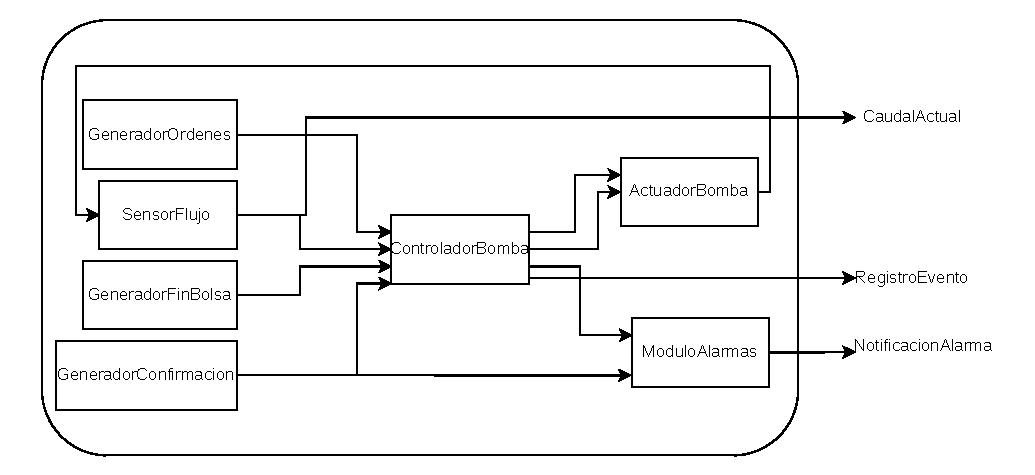
\includegraphics[width=\textwidth]{diagrama.pdf}
    \caption{Modelo Acoplado del Sistema de Bomba de Infusión}
    \label{fig:acoplado}
\end{figure}

\end{document}